% Template for PLoS
% Version 3.5 March 2018
%
% % % % % % % % % % % % % % % % % % % % % %
%
% -- IMPORTANT NOTE
%
% This template contains comments intended 
% to minimize problems and delays during our production 
% process. Please follow the template instructions
% whenever possible.
%
% % % % % % % % % % % % % % % % % % % % % % % 
%
% Once your paper is accepted for publication, 
% PLEASE REMOVE ALL TRACKED CHANGES in this file 
% and leave only the final text of your manuscript. 
% PLOS recommends the use of latexdiff to track changes during review, as this will help to maintain a clean tex file.
% Visit https://www.ctan.org/pkg/latexdiff?lang=en for info or contact us at latex@plos.org.
%
%
% There are no restrictions on package use within the LaTeX files except that 
% no packages listed in the template may be deleted.
%
% Please do not include colors or graphics in the text.
%
% The manuscript LaTeX source should be contained within a single file (do not use \input, \externaldocument, or similar commands).
%
% % % % % % % % % % % % % % % % % % % % % % %
%
% -- FIGURES AND TABLES
%
% Please include tables/figure captions directly after the paragraph where they are first cited in the text.
%
% DO NOT INCLUDE GRAPHICS IN YOUR MANUSCRIPT
% - Figures should be uploaded separately from your manuscript file. 
% - Figures generated using LaTeX should be extracted and removed from the PDF before submission. 
% - Figures containing multiple panels/subfigures must be combined into one image file before submission.
% For figure citations, please use "Fig" instead of "Figure".
% See http://journals.plos.org/plosone/s/figures for PLOS figure guidelines.
%
% Tables should be cell-based and may not contain:
% - spacing/line breaks within cells to alter layout or alignment
% - do not nest tabular environments (no tabular environments within tabular environments)
% - no graphics or colored text (cell background color/shading OK)
% See http://journals.plos.org/plosone/s/tables for table guidelines.
%
% For tables that exceed the width of the text column, use the adjustwidth environment as illustrated in the example table in text below.
%
% % % % % % % % % % % % % % % % % % % % % % % %
%
% -- EQUATIONS, MATH SYMBOLS, SUBSCRIPTS, AND SUPERSCRIPTS
%
% IMPORTANT
% Below are a few tips to help format your equations and other special characters according to our specifications. For more tips to help reduce the possibility of formatting errors during conversion, please see our LaTeX guidelines at http://journals.plos.org/plosone/s/latex
%
% For inline equations, please be sure to include all portions of an equation in the math environment.  For example, x$^2$ is incorrect; this should be formatted as $x^2$ (or $\mathrm{x}^2$ if the romanized font is desired).
%
% Do not include text that is not math in the math environment. For example, CO2 should be written as CO\textsubscript{2} instead of CO$_2$.
%
% Please add line breaks to long display equations when possible in order to fit size of the column. 
%
% For inline equations, please do not include punctuation (commas, etc) within the math environment unless this is part of the equation.
%
% When adding superscript or subscripts outside of brackets/braces, please group using {}.  For example, change "[U(D,E,\gamma)]^2" to "{[U(D,E,\gamma)]}^2". 
%
% Do not use \cal for caligraphic font.  Instead, use \mathcal{}
%
% % % % % % % % % % % % % % % % % % % % % % % % 
%
% Please contact latex@plos.org with any questions.
%
% % % % % % % % % % % % % % % % % % % % % % % %

\documentclass[10pt,letterpaper]{article}
\usepackage[top=0.85in,left=2.75in,footskip=0.75in]{geometry}

% amsmath and amssymb packages, useful for mathematical formulas and symbols
\usepackage{amsmath,amssymb}

% Use adjustwidth environment to exceed column width (see example table in text)
\usepackage{changepage}

% Use Unicode characters when possible
\usepackage[utf8x]{inputenc}

% textcomp package and marvosym package for additional characters
\usepackage{textcomp,marvosym}

% cite package, to clean up citations in the main text. Do not remove.
\usepackage{cite}

% Use nameref to cite supporting information files (see Supporting Information section for more info)
\usepackage{nameref,hyperref}

% line numbers
\usepackage[right]{lineno}

% ligatures disabled
\usepackage{microtype}
\DisableLigatures[f]{encoding = *, family = * }

% color can be used to apply background shading to table cells only
\usepackage[table]{xcolor}

% array package and thick rules for tables
\usepackage{array}

% code-listing package
\usepackage{minted}

% create "+" rule type for thick vertical lines
\newcolumntype{+}{!{\vrule width 2pt}}

% create \thickcline for thick horizontal lines of variable length
\newlength\savedwidth
\newcommand\thickcline[1]{%
  \noalign{\global\savedwidth\arrayrulewidth\global\arrayrulewidth 2pt}%
  \cline{#1}%
  \noalign{\vskip\arrayrulewidth}%
  \noalign{\global\arrayrulewidth\savedwidth}%
}

% \thickhline command for thick horizontal lines that span the table
\newcommand\thickhline{\noalign{\global\savedwidth\arrayrulewidth\global\arrayrulewidth 2pt}%
\hline
\noalign{\global\arrayrulewidth\savedwidth}}


% Remove comment for double spacing
%\usepackage{setspace} 
%\doublespacing

% Text layout
\raggedright
\setlength{\parindent}{0.5cm}
\textwidth 5.25in 
\textheight 8.75in

% Bold the 'Figure #' in the caption and separate it from the title/caption with a period
% Captions will be left justified
\usepackage[aboveskip=1pt,labelfont=bf,labelsep=period,justification=raggedright,singlelinecheck=off]{caption}
\renewcommand{\figurename}{Fig}

% Use the PLoS provided BiBTeX style
\bibliographystyle{plos2015}

% Remove brackets from numbering in List of References
\makeatletter
\renewcommand{\@biblabel}[1]{\quad#1.}
\makeatother



% Header and Footer with logo
\usepackage{lastpage,fancyhdr,graphicx}
\usepackage{epstopdf}
%\pagestyle{myheadings}
\pagestyle{fancy}
\fancyhf{}
%\setlength{\headheight}{27.023pt}
%\lhead{\includegraphics[width=2.0in]{PLOS-submission.eps}}
\rfoot{\thepage/\pageref{LastPage}}
\renewcommand{\headrulewidth}{0pt}
\renewcommand{\footrule}{\hrule height 2pt \vspace{2mm}}
\fancyheadoffset[L]{2.25in}
\fancyfootoffset[L]{2.25in}
\lfoot{\today}

%% Include all macros below

\newcommand{\lorem}{{\bf LOREM}}
\newcommand{\ipsum}{{\bf IPSUM}}

%% END MACROS SECTION


\begin{document}
\vspace*{0.2in}

% Title must be 250 characters or less.
\begin{flushleft}
{\Large
\textbf\newline{Parallelised Scalable Simulations of Biological Neural Networks using TensorFlow: A Beginners’ Guide} % Please use "sentence case" for title and headings (capitalize only the first word in a title (or heading), the first word in a subtitle (or subheading), and any proper nouns).
}
\newline
% Insert author names, affiliations and corresponding author email (do not include titles, positions, or degrees).
\\
Saptarshi Soham Mohanta\textsuperscript{1},
Collins Assisi\textsuperscript{1},
with Theoretical Neuroscience Group\textsuperscript{\textpilcrow}.
\\
\bigskip
\textbf{1} Indian Institute of Science Education and Research, Pune, Maharashtra, India
\\
\bigskip


% Current address notes
\textcurrency Current Address: Biology Department, Indian Institute of Science Education and Research, Pune, Maharashtra, India 

% Group/Consortium Author Note
\textpilcrow Membership list can be found in the Acknowledgments section.

% Use the asterisk to denote corresponding authorship and provide email address in note below.
* collins@iiserpune.ac.in

\end{flushleft}
% Please keep the abstract below 300 words
\section*{Abstract}
The dynamics of neurons and their networks have been studied extensively by modelling them as collections of differential equations, and the power of these mathematical tools are well recognised. Many tools and packages exist that allow the simulation of systems of neurons using these differential equations. However, there is a barrier of entry in terms of developing flexible general purpose simulations that are platform independent and support hardware acceleration on modern computing architectures such as GPUs/TPUs and Distributed Platforms. TensorFlow is a Python-based open-source package initially designed for machine learning algorithms, but it presents a scalable environment for a variety of computation including solving differential equations using iterative algorithms from numerical analysis such as Runge-Kutta methods. There are two significant benefits of such an implementation: high readability and scalability across a variety of computational devices. We explore the process of implementing a scalable simulation of a system of neurons based on Hodgkin-Huxley-like neuron equations using TensorFlow. We also discuss the limitations of such implementation and approaches to deal with them. 


% Please keep the Author Summary between 150 and 200 words
% Use first person. PLOS ONE authors please skip this step. 
% Author Summary not valid for PLOS ONE submissions.   
\section*{Author summary}
In the form of a 7-day tutorial, the reader is introduced to the mathematical modelling of neuronal networks based on the Hodgkin-Huxley Differential Equations and is instructed on developing highly parallelised but easily readable code for numerical methods such as Euler's Method and Runge-Kutta Methods to solve differential equations in Python and use them to simulate neuronal dynamics. To develop scalable code, Google's open-source package TensorFlow is introduced, and the reader is instructed in developing simulations using this package and handling the few limitations that come with this implementation. The reader is also introduced to coding structures that maximise the parallelizability of the simulation. Finally, the coding paradigm that was developed is used to simulate a model of Locus Antennal Lobe described in previous literature, and its efficacy is analysed. 

\linenumbers

% Use "Eq" instead of "Equation" for equation citations.
\section*{Motivation}
The processing of information by the nervous system spans across space and time, and mathematical modelling of these dynamics have found to be an essential tool. These models have been used extensively to study the dynamics and mechanisms of information processing at both the individual neuron level~\cite{} and the system of neurons level.~\cite{} These models generally utilise systems of simultaneous ordinary differential equations (ODEs) which are solved as initial value problems using well-studied methods from numerical analysis such as Euler's Method and Runge Kutta methods.~\cite{} From a detailed study of the mechanism of action of the neurons, ion channels, neurotransmitters or neuromodulators and their dynamics in different models,~\cite{} equations have been found that describe the behaviour of neurons and synapse. By forming interconnected systems of these individual groups of differential equations, the overall dynamics and behaviour of networks can be studied through deterministic or stochastic simulations which can be easily perturbed unlike the case for in vivo experiments.

A significant issue with such simulations is computational complexity. As the number of neurons increase, the number of possible synaptic connections increases quadratically. That is, for a system of $n$ neurons there can be at most $n^2$ different synapses of one type, each with its own set of equations. Thus, simulations can take very long times for large values of $n$. A solution to this problem is to implement some form of parallelisation in the ODE solver and the system of equations itself. One of the simplest methods of parallelizable computation is in the form of matrix algebra which can be accelerated using libraries such as BLAS which can only be used for accelerating CPU based computations. Similarly, CUDA is available for speeding up computations on Nvidia-based GPUs and TPUs.~\cite{} However, there is a barrier of entry to using low-level packages like CUDA for the general user as it sometimes requires an in-depth understanding of the architecture, particularly for troubleshooting.

This is where TensorFlow (an open-source Google product)~\cite{} gives us a massive edge. TensorFlow allows us much greater scalability and is way more flexible in terms of ease of implementation for specialised hardware. With minimal changes in the implementation, the code can be executed on a wide variety of heterogeneous and distributed systems ranging from mobile devices to clusters and specialised computing devices such as GPU and TPU cards. The modern advances in GPU/TPU design allow us to access even higher degrees of parallelisation. It is now even possible to have hundred of TeraFLOPS of computing power in a single small computing device. With TensorFlow, we can access these resources without even requiring an in-depth understanding of its architecture and technical knowledge of specific low-level packages like CUDA.

%~\cite{bib1}

\section*{How to use this Tutorial}

For this tutorial, the reader is expected to have an understanding of Python and some commonly used packages such as Numpy and Matplotlib. The reader is also expected to know some amount of calculus particularly the theory of differential equations. Access to a computer will the following prerequisite software/packages is preferable: Python 3.6 or above, Jupyter Notebook, Numpy Python package, Matplotlib Python package, and TensorFlow 1.13 or above. All software can be installed using Anaconda Distribution of Python 3. Instructions for TensorFlow installation is available on their website.

% For figure citations, please use "Fig" instead of "Figure". Fig~\ref{fig1}

% Place figure captions after the first paragraph in which they are cited.
%\begin{figure}[!h]
%\caption{{\bf Bold the figure title.}
%Figure caption text here, please use this space for the figure panel descriptions instead of using subfigure commands. A: Lorem ipsum dolor sit amet. B: Consectetur adipiscing elit.}
%\label{fig1}
%\end{figure}

\section*{Day 1: Of Numerical Integration and Python}
In this tutorial we are interested in solving ordinary differential equations of the form,
\begin{equation}
\frac{dx}{dt} = f(x, t)
\label{eq:ode}
\end{equation}
where, $x$ is an $N-$dimensional vector and $t$ typically stands for time. The function $f(x,t)$ may be a nonlinear function of $x$ that explicitly depends on $t$. In addition to specifying the form of the differential equation, one must also specify the value of $x$ at a particular time point. Say, $x=x_{0}$ at $t = t_0$. It is often not possible to derive a closed form solution for~\ref{eq:ode}. Therefore numerical methods to solve these equations are of great importance. One such example at the core of our tutorial are the Hodgkin-Huxley equations (ref) describing the dynamics of action potential generation and propagation in the giant axon of the squid. Alan Hodgkin and Andrew Huxley arrived at these equations after a series of clever experiments that tested the limits of experimental technology available at the time. It also tested the limits of computational tools available. The form of the differential equations they derived contained nonlinearities that made it analytically intractable. In order to compute action potentials, Huxley numerically intergrated the equations using a hand operated Bunsviga mechanical calculator. The calculation took nearly three weeks to complete (ref). They used a numerical method due to Hartree (ref 1932)integrate the differential equations. Each iteration that calculated the value of the solution at subsequent time points consisted of 9 steps. In calculating the solution over time, they also varied the step size such that dynamics occurring over faster time scales (such as the rising phase of the action potential) were calculated with time step sizes of $0.1-0.2$ms while slower dynamics (such as the small highly damped oscillation following a spike) was calculated with time steps that were an order of magnitude higher ($1$ms).

In this tutorial, we illustrate two numerical methods to iteratively compute each time step of the solution. The first is a simple one-step method known as the Euler's method of integration. The second is another popular method, the Runge-Kutta method of order 4 (abberviated as RK4) that is more accurrate than the Euler's method, but requires additional computations to calculate subsequent time steps. 

\subsection*{Euler's Method for Numerical Integration}
Our goal is to solve~\ref{eq:ode} - calculate $x(t)$ given an initial condition $x(t_n)=x_{n}$. The simplest method to solve~\ref{eq:ode} numerically is the Euler's method. Here we start from $x(t=t_{0})=x_{0}$ and compute the solution at subsequent time points ($t_{0}+\epsilon,t_{0}+2\epsilon,t_{0}+3\epsilon \dots $) iteratively. Each step of the computation is done using the same formula that can be derived by truncating a Taylor series after the first term. That is, the solution at time $t+\epsilon$ is given by,
\begin{equation}
x(t+\epsilon) = x_{0} + \epsilon\frac{dx}{dt} + \mathcal{O}(\epsilon^2)
\label{eq:euler}
\end{equation}
where $\frac{dx}{dt}=f(x,t)$. The higher order terms $\mathcal{O}(\epsilon^2)$ are ignored in this approximation. 

\begin{figure}
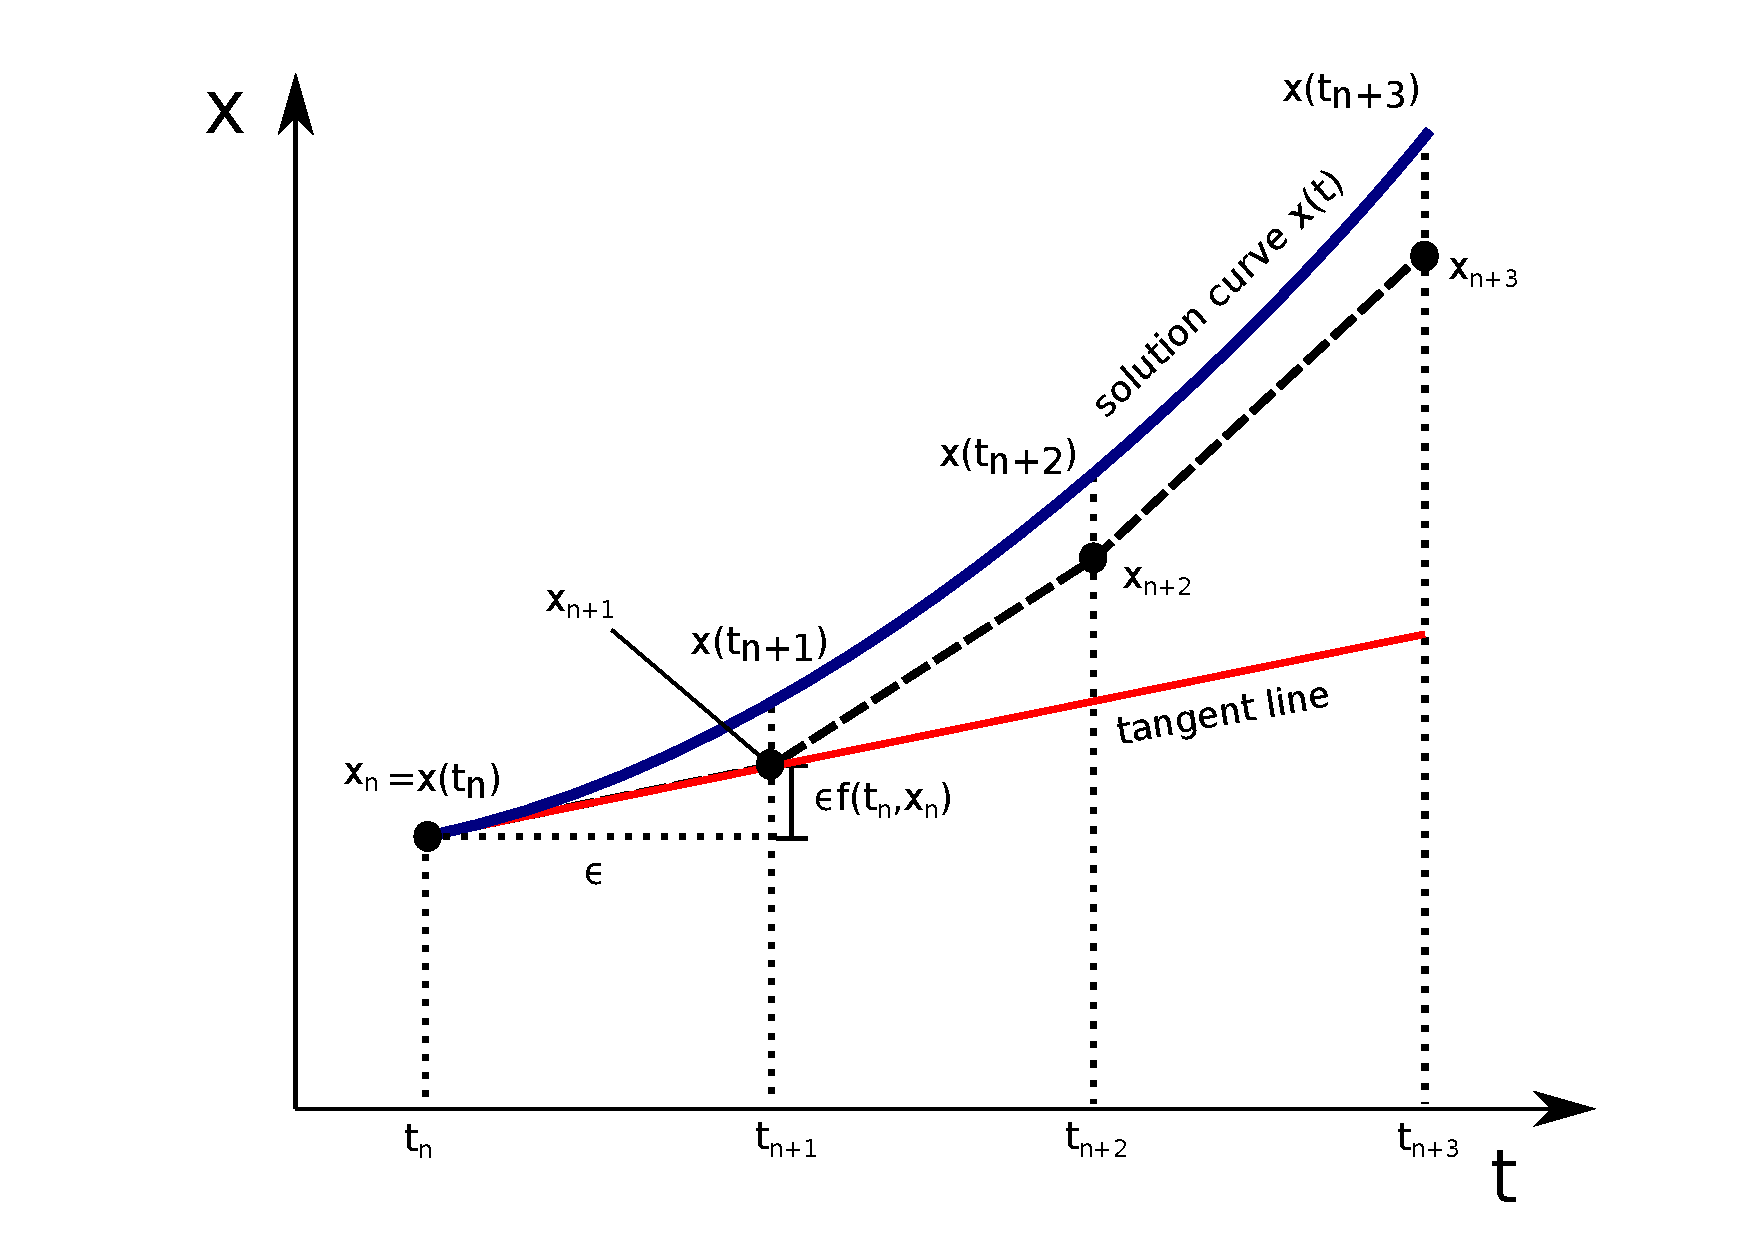
\includegraphics[scale=0.4]{Figures/fig1.pdf} 
\caption{Euler's method}
\label{fig:euler}
\end{figure}

A geometric interpretation of the Euler's method is shown in figure~\ref{fig:euler}. The solution of a particular differential equation is shown by the solid blue line in the figure. The dashed line approximates this solution by iteratively calculating $x$ at different time points using~\ref{eq:euler}. If the value of the solution at $t_{n}$ is $x_{n}$. $f(x_{n},t)$ is the slope of the tangent to the solution at $t_{n}$. If $\epsilon$ is sufficiently small, the solution at $t_{n+1}=t_{n}+\epsilon$ can be approximated by linearly extrapolating from $x_{n}$ to $x_{n} + \epsilon f(x_{n},t_{n})$

\subsection*{Implementation of Euler's Method in Python}

Let $\frac{dx}{dt}=5x$. We wish to calculate $x(t)$ over the interval $t\in[0,2)$  given the initial condition $x(0)=1$. The exact solution of this equation is $x(t) = e^{5t}$. In our implementation of Euler's method, we used the Python library Numpy to create and operate on arrays, and the plotting library Matplotlib, to display the results. We implement the Euler's Method in Python as follows:

\begin{minted}[linenos]{python}
import numpy as np
import matplotlib.pyplot as plt
def f(x,t): # define the function f(x,t)
    return 5*x
epsilon = 0.01 # define timestep
t = np.arange(0,2,epsilon) # define an array for t
x = np.zeros(t.shape) # define an array for x
x[0]= 1 # set initial condition
for i in range(1,t.shape[0]):
    x[i] = epsilon*f(x[i-1],t[i-1])+x[i-1] # Euler Integration Step
\end{minted}

\begin{figure}
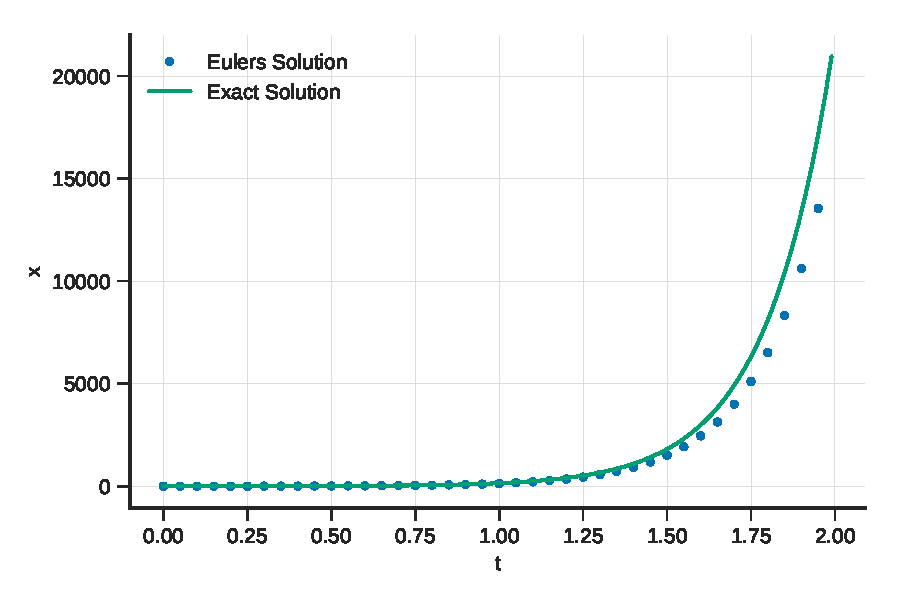
\includegraphics[scale=0.7]{Figures/fig2.pdf} 
\caption{Comparison of actual solution and approximation by Euler's method}
\label{fig:eulerError}
\end{figure}

The exact solution and the numerical solution are compared in Fig~\ref{fig:eulerError}. Notice that the approximation begins to diverge from the actual solution of the equation as the number of iterations increase. The omission of terms $\mathcal{O}(\epsilon^2)$ leads to a truncation error per step that can accumulate over time. 

\subsection*{Implementing Euler's method to solve a system of differential equations}

Euler's Method can also be easily applied to systems of equations. The Initial Value problem now becomes:

\begin{eqnarray}\frac{d\vec{X}}{dt} = \vec{f}(\vec{X}, t)\end{eqnarray}
\begin{eqnarray}\vec{X}(t_o) = \vec{X_o}\end{eqnarray}

where $\vec{X}=[X_1,X_2...]$ and $\vec{f}(\vec{X}, t)=[f_1(\vec{X}, t),f_2(\vec{X}, t)...]$. We rewrite Euler's method as:

\begin{eqnarray}t_{n+1} = t_n + \epsilon \end{eqnarray}
\begin{eqnarray}\vec{X}_{n+1} = \vec{X}_n + \epsilon \vec{f}(\vec{X}_n, t_n)\end{eqnarray}

Let $\frac{d\vec{X}}{dt}=f(\vec{X},t)$, we wish to find $\vec{X}(t)$ over $t\in[0,2)$, given that $\vec{X}(t)=[x,y]$, $\vec{X}(0)=[1,0]$ and $f(\vec{X},t) = [x-y,y-x]$. We implement the modified algorithm as follows:

\begin{minted}[linenos]{python}
def f(X,t): # the function f(X,t) now takes a vector X as input
    x,y = X #the first and the second elements of X are assigned to x and y
    return np.array([x-y,y-x])
t = np.arange(0,2,epsilon) # define an array for t
X = np.zeros((2,t.shape[0])) # initialize an array for X
X[:,0]= [1,0] # set initial condition
for i in range(1,t.shape[0]):
    X[:,i] = epsilon*f(X[:,i-1],t[i-1])+X[:,i-1] # Euler Integration Step
\end{minted}

\subsection*{A generalized code implementing the Euler method}
Here we rewrite the code in a modular fashion and cast the integrator as a function that takes in 3 inputs ie. the function $\vec{f}(\vec{y},t)$ where $\frac{d\vec{y}}{dt}=f(\vec{y},t)$, the time array, and initial vector $\vec{y}_{0}$. We will find this form to be particularly useful when we use tensorflow constructs to code the integrator. Further, it allows us to write multiple integrating functions (for example Euler or RK4) within the same class and call a specific integrator as needed. In addition we also introduce a function to ensure that the correct inputs are given to the integrator failing which an error message is generated. 

\subsubsection*{Algorithm}

\begin{itemize}
\item Get the required inputs: function $\vec{f}(\vec{y},t)$, initial condition vector $\vec{y}_0$ and time series $t$. Entering a time series $t$ allows for greater control over $\epsilon$ as it can now vary for each timestep. 
\item Check if the input is of the correct datatype ie. floating point decimal.
\item Create a zero matrix to hold the output.
\item For each time step, perform the update $\vec{y}$ using the Euler method with variable $\epsilon$ and store it in the output matrix.
\item Return the output time series [number of equations $\times$ iterations] matrix.
\end{itemize}

\begin{minted}[linenos]{python}
def check_type(y,t): # Ensure Input is Correct
    return y.dtype == np.floating and t.dtype == np.floating
class _Integrator():
    def integrate(self,func,y0,t):
        time_delta_grid = t[1:] - t[:-1]
        y = np.zeros((y0.shape[0],t.shape[0]))
        y[:,0] = y0
        for i in range(time_delta_grid.shape[0]):
            y[:,i+1]= time_delta_grid[i]*func(y[:,i],t[i])+y[:,i]
        return y
def odeint_euler(func,y0,t):
    y0 = np.array(y0)
    t = np.array(t)
    if check_type(y0,t):
        return _Integrator().integrate(func,y0,t)
    else:
        print("error encountered")
solution = odeint_euler(f,[1.,0.],t)
\end{minted}

\subsection*{Runge-Kutta Methods for Numerical Integration}

Euler's method $x_{n+1}=x_n + \epsilon f(x_n,t_n)$ calculates the solution at $t_{n+1}=t_n+\epsilon$ given the solution at $t_n$. In doing so we use the derivative at $t_{n}$ though its value may change throughout the interval $[t,t+\epsilon]$.  This results in an error in the order of $\mathcal{O}(\epsilon^2)$. By calculating the derivatives at intermediate steps, one can reduce the error at each step. Consider the following second order method where the slope is calculated at $t_{n}$ and $t_n+\frac{\epsilon}{2}$.

\begin{eqnarray}k_1=\epsilon f(x_n,t_n)\end{eqnarray}
\begin{eqnarray}k_2=\epsilon f(x_n+\frac{k_1}{2},t_n+\frac{\epsilon}{2})\end{eqnarray}
\begin{eqnarray}x_{n+1}=x_n+k_2+O(\epsilon^3)\end{eqnarray}


This method is called the second order Runge-Kutta method or the midpoint method.
\begin{figure}
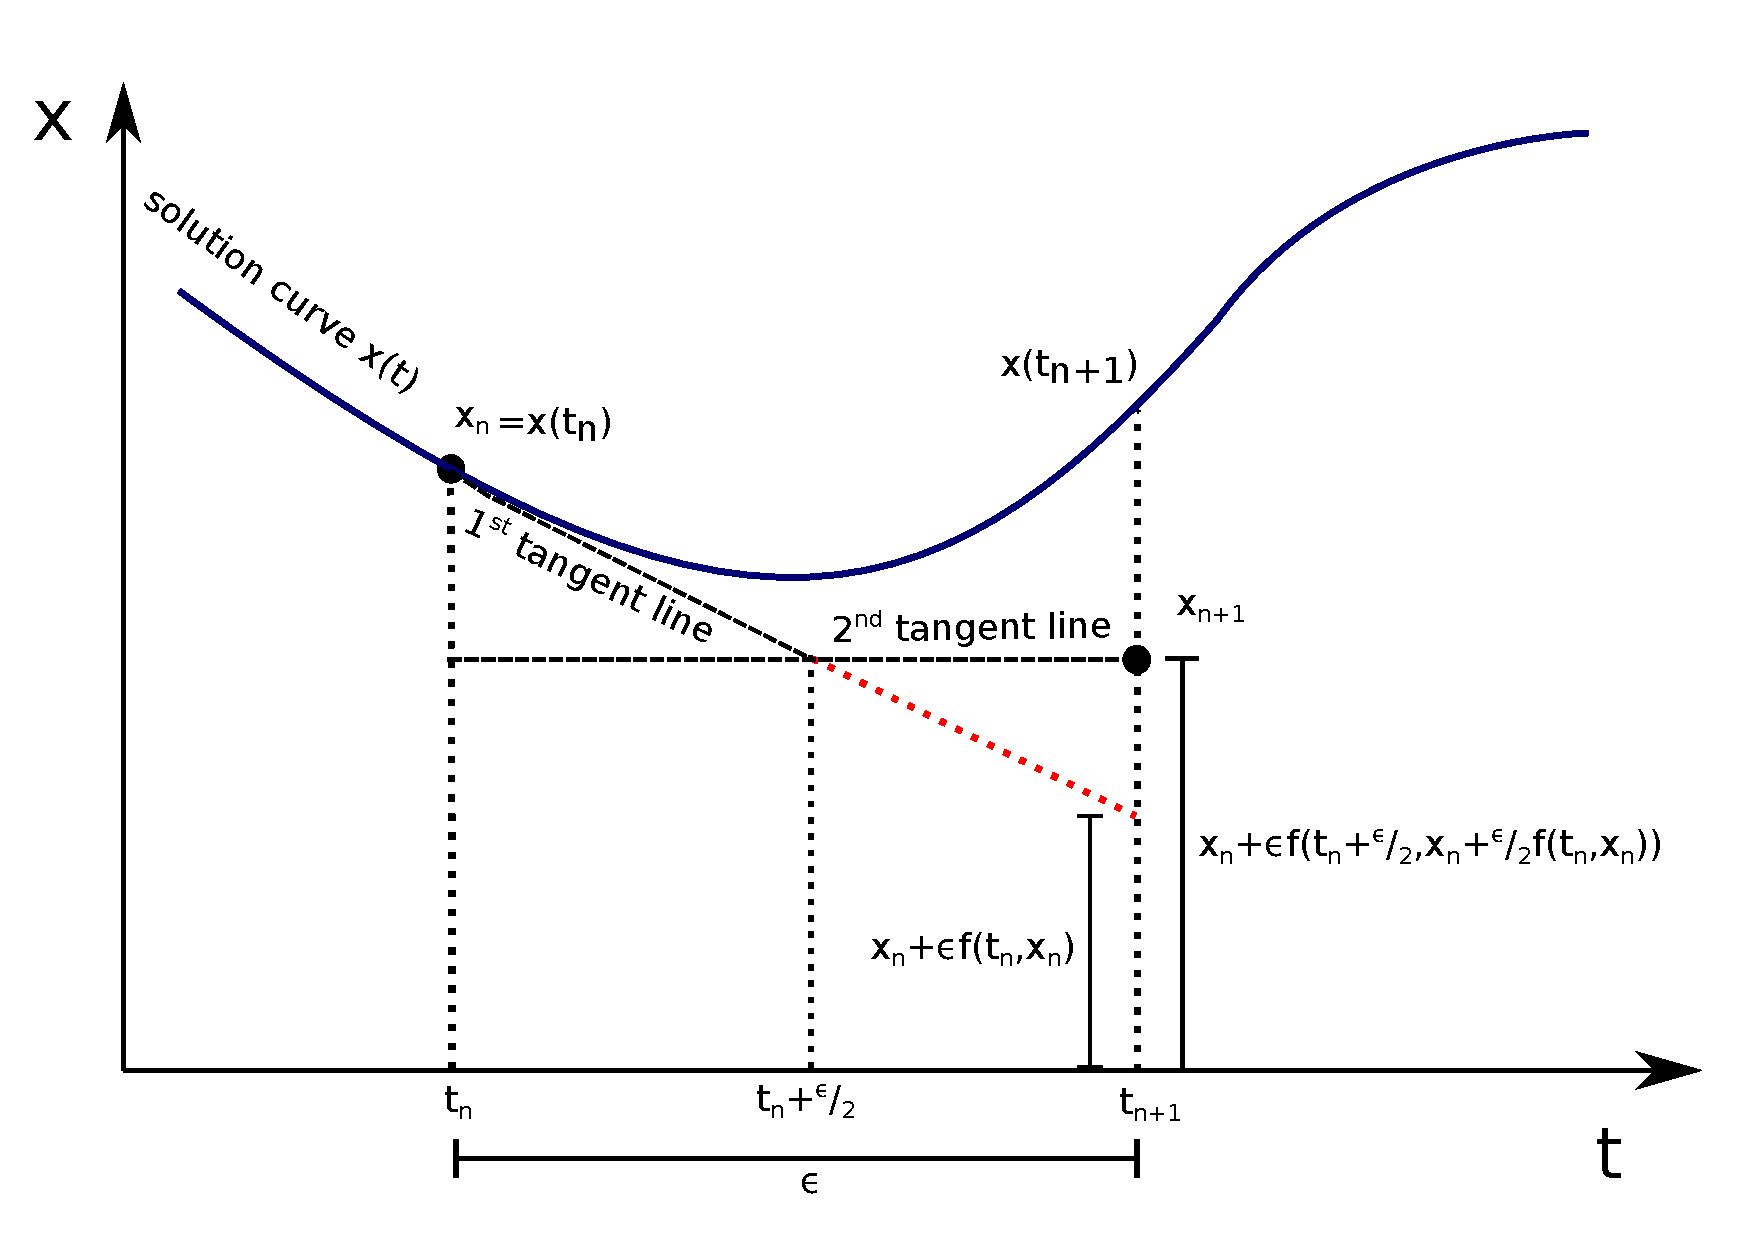
\includegraphics[scale=0.4]{Figures/fig4.pdf} 
\caption{Second order Runge-Kutta method}
\label{fig:RK2}
\end{figure}
Figure~\ref{fig:RK2} is a schematic description of the second order Runge-Kutta methd. The blue curve denotes a solution of some differential equation. The goal is to calculate 

But we do not have to stop here. By further rewriting the equation, we can cancel higher order error terms and reach the most commonly used fourth-order Runge-Kutta Methods or RK4 method, which is described below:

\begin{eqnarray}k_1=f(x_n,t_n)\end{eqnarray}
\begin{eqnarray}k_2=f(x_n+\epsilon\frac{k_1}{2},t_n+\frac{\epsilon}{2})\end{eqnarray}
\begin{eqnarray}k_3=f(x_n+\epsilon\frac{k_2}{2},t_n+\frac{\epsilon}{2})\end{eqnarray}
\begin{eqnarray}k_4=f(x_n+\epsilon k_3,t_n+\epsilon)\end{eqnarray}
\begin{eqnarray}y_{n+1}=y_n+\frac{\epsilon}{6}(k_1+2 k_2+2 k_3+k_4)+\mathcal{O}(\epsilon^5)\end{eqnarray}

Note that this numerical method is again easily converted to a vector algorithm by simply replacing $x_i$ by the vector $\vec{X_i}$. This method is what we will use to simulate our networks.


\subsection*{Generalized RK4 Method in Python}

We can now modify the Euler Integration code implemented earlier iwith a generalized function for RK4 that takes three inputs \textemdash the function $f(\vec{y},t)$ when $\frac{d\vec{y}}{dt}=f(\vec{y},t)$, the time array, and an initial vector $\vec{y_0}$. The code can be updated as follows,

\begin{minted}[linenos]{python}
# RK4 Integration Steps replace the Euler's Updation Steps
k1 = func(y[:,i], t[i])                               
half_step = t[i] + time_delta_grid[i] / 2
k2 = func(y[:,i] + time_delta_grid[i] * k1 / 2, half_step)
k3 = func(y[:,i] + time_delta_grid[i] * k2 / 2, half_step)
k4 = func(y[:,i] + time_delta_grid[i] * k3, t + time_delta_grid[i])
y[:,i+1]= (k1 + 2 * k2 + 2 * k3 + k4) * (time_delta_grid[i] / 6) + y[:,i]
\end{minted}

As an \textbf{Exercise}, try to solve the equation of a simple pendulum and observe its dynamics using Euler Method and RK4 methods. The equation of motion of a simple pendulum is given by: 

\begin{eqnarray}\frac{d^2s}{dt^2}=L\frac{d^2\theta}{dt^2}=-g\sin{\theta}\end{eqnarray}

where $L$ = Length of String and $\theta$ = angle made with vertical. To solve this second order differential equation you may use a dummy variable $\omega$ representing angular velocity such that:

\begin{eqnarray}\frac{d\theta}{dt}=\omega \end{eqnarray}
\begin{eqnarray}\frac{d\omega}{dt}=-\frac{g}{L}\sin{\theta} \end{eqnarray}

\section*{Day 2: Let the Tensors Flow!}

\subsection*{An Introduction to TensorFlow}

TensorFlow is an open-source software library that was developed by the researchers and engineers in the Google Brain team, primarily for machine learning applications. However, the system is general enough to be applicable in a number of other domains as well.~\cite{}.  Its flexible architecture allows one to perform computations on a number of different platforms \textemdash CPUs, GPUs , TPUs and clusters of servers. 

\subsection*{Why GPU/TPU vs CPU?}

The answer lies in the architecture Fig~\ref{}:  
\begin{itemize}
\item CPU = Faster per Core Processing, Slow but Large Memory Buffer, Few Cores
\item GPU/TPU = Slower Processing, Faster but Smaller Memory Buffer, Many Cores
\end{itemize}

Thus GPUs and TPUs are optimized for large number of simple calculations done parallely. The extent of this  parallelization makes it suitable for vector/tensor manipulation.

\subsection*{How TensorFlow works?}

TensorFlow essentially performs numerical computations on multidimensional arrays (called tensors) using "data flow graphs" or "computation graphs". In these graphs, nodes represent variables/placeholders/constants or mathematical operations such as matrix multiplication or elementwise addition and the edges in the graph represent the flow of tensors between operations (nodes). Tensor is the central unit of data in TensorFlow giving the package its name. For example, look at the following computation graph in Fig~\ref{} where "matmul" is the node which represents the matrix multiplication operation. a and b are input matrices (2-D tensors) and c is the resultant matrix.

\subsection*{Implementing a computation graph in TensorFlow}

\begin{minted}[linenos]{python}
# Creating nodes in the computation graph 
a = tf.constant([[1.],[2.],[3.]], dtype=tf.float64) # a 3x1 column matrix 
b = tf.constant([[1.,2.,3.]], dtype=tf.float64) # a 1x3 row matrix 
c = tf.matmul(a, b) 
# To run the graph, we need to create a session.
# Creating the session initializes the computational device.
sess = tf.Session() # start a session
output = sess.run(c) # compute the value of c
sess.close() # end the session
print(output)
# TO automatically close the session after computation, Use:
# with tf.Session() as sess:
#    output = sess.run(c) 
\end{minted}

\subsection*{Iterating recursively over lists/arrays in TensorFlow}

Say, one wants to recursively apply a function on an initial value but the function takes in additional input at every recursive call, for example, to find a cumulative sum over a list. Every step is addition of the new element from the list onto the last addition. The TensorFlow function tf.scan allows us to easily implement such an iterator.

\begin{minted}[linenos]{python}
# define the recursive function that takes in two values the
# accumulated value and the additional input from a list.
def recursive_addition(accumulator,new_element):
    return accumulator+new_element
# define the list over which we iterate
elems = np.array([1, 2, 3, 4, 5, 6])
# tf.scan takes in three inputs: the recursive function, the 
# list to iterate over and the initial value. If an initial 
# value is not provided, its taken as the first element of elems.
# accumulate with no initializer
cum_sum_a = tf.scan(recursive_addition, elems) 
# accumulate with initializer as the number 5
cum_sum_b = tf.scan(recursive_addition, elems, tf.constant(5,dtype=tf.int64))
with tf.Session() as sess:
    output_a = sess.run(cum_sum_a)
    output_b = sess.run(cum_sum_b)
print(output_a)
print(output_b)
# This prints :
#[ 1  3  6 10 15 21]
#[ 6  8 11 15 20 26]
\end{minted}

As an \textbf{Exercise} try using tf.scan to compute the fibonacci sequence. One may have noticed that our integration is essentially an recursive process over the time series. Both the updation rules can just be written as a recursive function $F$ such that $X_{i+1}=F(X_i,t_i,\epsilon_i)$. We would want our output to be the array $[X_0,F(X_0,t_0,\epsilon_0),F(F(X_0,t_0,\epsilon_0),t_1,\epsilon_1)...]$. To get this, we just need to recursively iterate over the array of time and $\epsilon$ and apply a updation function $F$ recursively on the initial condition, which exactly what tf.scan enables us to do.

\subsection*{Euler Integration Function in TensorFlow}

Transitioning to TensorFlow is not a trivial process, but once you get a gist of how it works, it is as simple as using numpy. Because of the way the TensorFlow architecture is designed, there are a few limitations to how one can do simpler operations/manipulation. But it is easy to overcome using the correct function and code patterns which can be easily learnt.

\begin{minted}[linenos]{python}
def tf_check_type(t, y0): # Ensure Input is Correct
    if not (y0.dtype.is_floating and t.dtype.is_floating): 
        # The datatype of any tensor t is accessed by t.dtype
        raise TypeError('Error in Datatype')
class _Tf_Integrator():
    def integrate(self, func, y0, t): 
        time_delta_grid = t[1:] - t[:-1]  
        def scan_func(y, t_dt): 
            t, dt = t_dt
            dy = dt*func(y,t)
            return y + dy
        # iterating over (a,b) where a and b are lists of same size
        # results in the ith accumulative step in tf.scan receiving
        # the ith elements of a and b zipped together
        y = tf.scan(scan_func, (t[:-1], time_delta_grid),y0) 
        return tf.concat([[y0], y], axis=0)
def tf_odeint_euler(func, y0, t):
    # Convert input to TensorFlow Objects
    t = tf.convert_to_tensor(t, preferred_dtype=tf.float64, name='t')
    y0 = tf.convert_to_tensor(y0, name='y0')
    tf_check_type(y0,t)
    return _Tf_Integrator().integrate(func,y0,t)
    
# Define a function using Tensorflow math operations. 
# This creates the computation graph.
def f(X,t):
    # extracting a single value eg. X[0] returns a single value but
    # we require a tensor, so we extract a range with one element.
    x = X[0:1] 
    y = X[1:2]
    out = tf.concat([x-y,y-x],0)
    return out
y0 = tf.constant([1,0], dtype=tf.float64)
epsilon = 0.01
t = np.arange(0,2,epsilon)
# Define the final value (output of scan) that we wish to compute
state = tf_odeint_euler(f,y0,t)
# Start a TF session and evaluate state
with tf.Session() as sess:
    state = sess.run(state)
\end{minted}

\subsection*{RK4 Integration Function in TensorFlow}

Now, we implement the exact same RK4 integrator in TensorFlow, thus we make a small change in the integrate function. Also to make the code more modular, we introduce the differential step calculator to a different function, everything else remains the same.

\begin{minted}[linenos]{python}
def integrate(self, func, y0, t): 
        time_delta_grid = t[1:] - t[:-1]
        def scan_func(y, t_dt): 
            t, dt = t_dt
            dy = self._step_func(func,t,dt,y) # Make code more modular.
            return y + dy
        y = tf.scan(scan_func, (t[:-1], time_delta_grid),y0)
        return tf.concat([[y0], y], axis=0)
    def _step_func(self, func, t, dt, y):
        k1 = func(y, t)
        half_step = t + dt / 2
        dt_cast = tf.cast(dt, y.dtype) # Failsafe
        k2 = func(y + dt_cast * k1 / 2, half_step)
        k3 = func(y + dt_cast * k2 / 2, half_step)
        k4 = func(y + dt_cast * k3, t + dt)
        return tf.add_n([k1, 2 * k2, 2 * k3, k4]) * (dt_cast / 6)
\end{minted}

As an \textbf{Exercise}, try to simulate the non-linear Lorentz Attractor using Euler Method and RK4 on TensorFlow which is given by the equations:

\begin{eqnarray}\frac{dx}{dt}=\sigma(y-x) \end{eqnarray}
\begin{eqnarray}\frac{dy}{dt}=x(\rho-z)-y \end{eqnarray}
\begin{eqnarray}\frac{dz}{dt}=xy-\beta z \end{eqnarray}

Use the values $\sigma =10$, $\beta =\frac{8}{3}$, $\rho =28$. You can try simulating this system at two nearby starting conditions and comment on the difference.

\section*{Day 3: Cells in Silicon}

We start with our discussion with the Hodgkin Huxley Neurons and how we can simulate them in python using Tensorflow and Numerical Integration.

\subsection*{What is the Hodgkin Huxley Neuron Model?}

Hodgkin and Huxley performed many experiments on the giant axon of the squid and found three different types of ion currents - sodium, potassium, and a leak current. They found that specific voltage-dependent ion channels, for sodium and for potassium, control the flow of those ions through the cell membrane from different electrophysiology studies involving phamacological blocking of ion channels. The leak current essentially takes care of other channel types which are not described explicitly. 

The Hodgkin-Huxley model of neurons can easily be understood with the help of a RC circuit diagram.(Fig) The semipermeable cell membrane separates the interior of the cell from the extracellular liquid and acts as a capacitor. If an input current I(t) is injected into the cell, it may add further charge on the capacitor, or leak through the channels in the cell membrane. Because of active ion transport through the cell membrane, the ion concentration inside the cell is different from that in the extracellular liquid. The Nernst potential generated by the difference in ion concentration is represented by a battery.

We now convert the above considerations into mathematical equations. The conservation of electric charge on a piece of membrane implies that the applied current $I(t)$ may be split in a capacitive current $I_C$ which charges the capacitor $C_m = 1 \mu F/cm^2$ and further components $I_k$ which pass through the ion channels. Thus $I(t) = I_C(t) + \sum_kI_k(t)$ where the sum runs over all ion channels. 

In the standard Hodgkin-Huxley model, there are only three types of channel: a Sodium channel, a Potassium channel and an unspecific leakage channel. From the definition of a capacitance $C_m=\frac{q}{u}$, $I_C=C_m\frac{du}{dt}$ where $q$ is a charge and $u$ the voltage across the capacitor. Thus the model becomes:

\begin{eqnarray}\label{d3_1}C_m\frac{du}{dt}=−I_{Na}(t)−I_{K}(t)−I_{L}(𝑡)+I(t)\end{eqnarray}

In biological terms, $u$ is the voltage across the membrane. Hogkin and Huxley found the Na and K ion currents to be dependent on the voltage and of the form given below:

\begin{eqnarray}\label{d3_2}I_{Na} = g_{Na}m^3h(u−E_{Na})\end{eqnarray}
\begin{eqnarray}\label{d3_3}I_K = g_Kn^4(u−E_K)\end{eqnarray}
\begin{eqnarray}\label{d3_4}I_L = g_L(u−E_L)\end{eqnarray}

where $E_{Na}=50\ mV$, $E_K = -95\ mV$ and $E_L=-55\ mV$ are the reversal potentials; $g_{Na} = 100\ \mu S/cm^2$, $g_K = 10\ \mu S/cm^2$ and $g_L = 0.15\ \mu S/cm^2$ are the channel conductances; and m,h, and n are gating variables that follow the dynamics given by:

\begin{eqnarray}\label{d3_5}\frac{dm}{dt} = - \frac{1}{\tau_m}(m-m_0)\end{eqnarray}
\begin{eqnarray}\label{d3_6}\frac{dh}{dt} = - \frac{1}{\tau_h}(h-h_0)\end{eqnarray}
\begin{eqnarray}\label{d3_7}\frac{dn}{dt} = - \frac{1}{\tau_n}(n-n_0)\end{eqnarray}

where $\tau_m$, $\tau_h$ and $\tau_n$ are voltage dependent time constants and $m_0$, $h_0$ and $n_0$ are voltage dependent asymptotic gating values. These functions are empirically determined for different types of neurons. For an example, take a look at figure.

\subsection*{Implementing the Dynamical Function for an Hodkin Huxley Neuron}

For integration, we will use the TensorFlow RK4 integrator that we created. A simple Hodgkin Huxley Neuron has a 4 main dynamical variables: V = Membrane Potential, m = Sodium Activation Gating Variable, h = Sodium Inactivation Gating Variable, and n = Potassium Channel Gating Variable. And the dynamics are given by Eq~(\ref{d3_1}), Eq~(\ref{d3_5}),Eq~(\ref{d3_6}) and Eq~(\ref{d3_7}) where the values of $\tau_m$, $\tau_h$, $\tau_n$, $m_0$, $h_0$, $n_0$ are given empirically derived formulae (Fig) and channel currents are determined by Eq~(\ref{d3_2}),Eq~(\ref{d3_3}) and Eq~(\ref{d3_4}).

\begin{minted}[linenos]{python}
# Step 1: Defining Parameters of the Neuron 
C_m = 1
g_K = 10
E_K = -95
g_Na = 100
E_Na = 50 
g_L = 0.15
E_L = -55
# Step 2: Defining functions to calculate tau_x and x_0
# Note: Always use TensorFlow functions for all operations.
def K_prop(V):
    T = 22
    phi = 3.0**((T-36.0)/10)
    V_ = V-(-50)
    alpha_n = 0.02*(15.0 - V_)/(tf.exp((15.0 - V_)/5.0) - 1.0)
    beta_n = 0.5*tf.exp((10.0 - V_)/40.0) 
    t_n = 1.0/((alpha_n+beta_n)*phi)
    n_0 = alpha_n/(alpha_n+beta_n)
    return n_0, t_n
def Na_prop(V):
    T = 22
    phi = 3.0**((T-36)/10)
    V_ = V-(-50)
    alpha_m = 0.32*(13.0 - V_)/(tf.exp((13.0 - V_)/4.0) - 1.0)
    beta_m = 0.28*(V_ - 40.0)/(tf.exp((V_ - 40.0)/5.0) - 1.0)
    alpha_h = 0.128*tf.exp((17.0 - V_)/18.0)
    beta_h = 4.0/(tf.exp((40.0 - V_)/5.0) + 1.0)
    t_m = 1.0/((alpha_m+beta_m)*phi)
    t_h = 1.0/((alpha_h+beta_h)*phi)
    m_0 = alpha_m/(alpha_m+beta_m)
    h_0 = alpha_h/(alpha_h+beta_h)
    return m_0, t_m, h_0, t_h
# Step 3: Defining function that calculate Neuronal currents
def I_K(V, n):
    return g_K  * n**4 * (V - E_K)
def I_Na(V, m, h):
    return g_Na * m**3 * h * (V - E_Na)
def I_L(V):
    return g_L * (V - E_L)
# Step 4: Define the function dX/dt where X is the State Vector
def dXdt(X, t):
    V = X[0:1]
    m = X[1:2]
    h = X[2:3]
    n = X[3:4]
    dVdt = (5 - I_Na(V, m, h) - I_K(V, n) - I_L(V)) / C_m 
    # Here the current injection I_injected = 5 uA
    m0,tm,h0,th = Na_prop(V)
    n0,tn = K_prop(V)
    dmdt = - (1.0/tm)*(m-m0)
    dhdt = - (1.0/th)*(h-h0)
    dndt = - (1.0/tn)*(n-n0)
    out = tf.concat([dVdt,dmdt,dhdt,dndt],0)
    return out
# Step 5: Define Initial Condition and Integrate
y0 = tf.constant([-71,0,0,0], dtype=tf.float64)
epsilon = 0.01
t = np.arange(0,200,epsilon)
state = odeint(dXdt,y0,t)
with tf.Session() as sess:
    state = sess.run(state)
\end{minted}

\subsection*{Simulating Multiple Independent HH Neurons at the Same Time}

Although, simulating a Single Hodgkin-Huxley Neuron is possible in TensorFlow, the real ability of tensorflow can be seen only when a large number of simultaneous diffential equations are to be solved at the the same time. Let's try to simulate 20 independent HH neurons with different input currents and characterise the firing rates. 

\subsubsection*{Methods of Parallelization}
TensorFlow has the intrinsic ability to speed up any and all Tensor computations using available multi-cores, and GPU/TPU setups. There are two major parts of the code where TensorFlow can help us really speed up the computation:
\begin{enumerate}
\item \textbf{RK4 Steps:} Since the TensorFlow implementation of the Integrator utilizes Tensor calculations, TensorFlow will automatically speed it up.
\item \textbf{Functional Evaluations:} Looking at Dynamical Equations that describe the neuronal dynamics, its easy to notice that all simple HH Neurons share the same or atleast similar dynamical equations but will vary only in the values of parameters. We can exploit this to speed up the computations.
\end{enumerate}

Say $\vec{X}=[V,m,n,h]$ is the state vector of a single neuron and its dynamics are defined using parameters $C_m,g_K,...E_L$ equations of the form: 

\begin{eqnarray}\frac{d\vec{X}}{dt} = [f_1(\vec{X},C_m,g_K,...E_L),f_2(\vec{X},C_m,g_K,...E_L)...f_m(\vec{X},C_m,g_K,...E_L)]\end{eqnarray}

We have to somehow convert these to a form in which all evaluations are done as vector calculations and NOT scalar calculations.

So, what we need for a system of n neurons is to have a method to evaluate the updation of $\mathbf{X}=[\vec{X_1},\vec{X_2}...\vec{X_n}]$ where $\vec{X_i}=[V_1,m_1,n_1,h_1]$ is the state vector of the $i$th neuron. Now there is a simple trick that allows us to maximize the parallel processing. Each neuron represented by $\vec{X_i}$ has a distinct set of parameters and differential equations.

Now, despite the parameters being different, the functional forms of the updation is similar for the same state variable for different neurons. Thus, the trick is to reorganize $\mathbf{X}$ as $\mathbf{X'}=[(V_1,V_2,...V_n),(m_1,m_2,...m_n),(h_1,h_2,...h_n),(n_1,n_2,...n_n)]=[\vec{V},\vec{m},\vec{h},\vec{n}]$. And the parameters as $\vec{C_m},\vec{g_K}$ and so on.

Now that we know the trick, what is the benefit? Earlier, each state variable (say $V_i$) had a DE of the form:

\begin{eqnarray}\frac{dV_i}{dt}=f(V_i,m_i,h_i,n_i,C_{m_i},g_{K_i}...)\end{eqnarray}

This is now easily parallelizable using a vector computation of a form: 

\begin{eqnarray}\frac{d\vec{V}}{dt}=f(\vec{V},\vec{m},\vec{h},\vec{n},\vec{C_m},\vec{g_K}...)\end{eqnarray}

Thus we can do the calculations as:
\begin{eqnarray}\frac{d\mathbf{X'}}{dt}= \Big[\frac{d\vec{V}}{dt},\frac{d\vec{m}}{dt},\frac{d\vec{h}}{dt},\frac{d\vec{n}}{dt}\Big]\end{eqnarray}

\subsubsection*{Implementation}

Notice that the functions calculating gating dynamics and channel currents already are capable of vector input and output, so we do not need to change them. What we do need to change is the parameters which should now be vectors, the differential evaluation  function which should now be designed to handle grouped parameters, and finally the initial condition.

\begin{minted}[linenos]{python}
n_n = 20 # number of simultaneous neurons to simulate
# parameters will now become n_n-vectors
C_m = [1.0]*n_n
g_K = [10.0]*n_n
E_K = [-95.0]*n_n
g_Na = [100]*n_n
E_Na = [50]*n_n 
g_L = [0.15]*n_n
E_L = [-55.0]*n_n

# The state vector definition will change
def dXdt(X, t):
    V = X[:1*n_n]       # First n_n values are Membrane Voltage
    m = X[1*n_n:2*n_n]  # Next n_n values are Sodium Activation Gating
    h = X[2*n_n:3*n_n]  # Next n_n values are Sodium Inactivation Gating
    n = X[3*n_n:]       # Last n_n values are Potassium Gating
    dVdt = (np.linspace(0,10,n_n)-I_Na(V, m, h)-I_K(V, n)-I_L(V))/ C_m 
    # Input current is linearly varied between 0 and 10
    m0,tm,h0,th = Na_prop(V)
    n0,tn = K_prop(V)
    dmdt = - (1.0/tm)*(m-m0)
    dhdt = - (1.0/th)*(h-h0)
    dndt = - (1.0/tn)*(n-n0)
    out = tf.concat([dVdt,dmdt,dhdt,dndt],0)
    return out
y0 = tf.constant([-71]*n_n+[0,0,0]*n_n, dtype=tf.float64)
\end{minted}

The output can be seen in Fig.

\subsection*{Quantifying the Firing Rates against Input Current}

One way to quantify the firing rate is to perform a fourier analysis and find peak frequency, but an easier way to find the rate is to see how many times it crosses a threshold say 0 mV in a given time, here it is for 200ms = 0.2s, and find the rate. The output can be seen in Fig.

\begin{minted}[linenos]{python}
rate = np.bitwise_and(state[:-1,:20]<0,state[1:,:20]>0).sum(axis=0)/0.2
\end{minted}

\section*{Day 4: Neurons and Networks}
In this section we simulate a network of neurons interacting via synapses. Each synapse is defined by its own set of state variables and differential equations governing their temporal evolution. There are different kinds of synapses - electrical and chemical synapse. Electrical synapses are essentially physical conduits that allow the flow of ions across connected neurons. Chemical synapses are more common in the brain and are more complex than electrical synapses. When an action potential arrives at the axon terminal, it leads to the opening of voltage-gated calcium channels. The incoming calcium triggers neurotransmitter filled vesciles to fuse with the axon terminal membrane and release their cargo into the synaptic cleft. The neurotransmitters diffuse across the cleft and open (or close) ion channels on the post-synaptic neuron. This can cause a depolarization (increase in potential across the post-synaptic neuron's membrane) that makes it easier for the neuron to spike or it can inhibit the neuron and have the opposite effect. In some cases these effects are direct in that a neurotransmitter binds to a receptor in the post-synaptic site and causes deviations in membrane potential. The effect of a synapse can also be indirect such that neurotransmitters invoke a second messenger cascade that eventually leads to the opening or closing of ion channels in the post-synaptic neuron. Here we model excitatory and inhibitory chemical synapses.The network of interactions between neurons will be described by a connectivity matrix. Each type of synapse will have its own connectivity matrix.

\subsubsection*{Modelling Synapses}

The current ($I_{syn}$)that passes through a synaptic channel depends on the difference between its reversal potential ($E_{syn}$) and the actual value of the membrane potential ($u$), and is $I_{syn}(t)=g_{syn}(t)(u(t)−E_{syn})$. We can describe the synaptic conductance $g_{syn}(t)=g_{max}[O](t)$, by its maximal conductance $g_{max}$ and a gating variable $[O]$, where $[O](𝑡)$ is the fraction of open synaptic channels. Channels open when a neurotransmitter binds to the synapse which is a function of the presynaptic activation $[T]$.

\begin{eqnarray}\label{d4_1}\frac{d[O]}{dt}=\alpha[T](1−[O])−\beta[O]\end{eqnarray}

where $\alpha$ is the binding constant, $\beta$ the unbinding constant and $(1−[O])$ the fraction of closed channels where binding of neurotransmitter can occur. The functional form of T depends on the type and nature of the synapse.
	

\subsubsection*{Acetylcholine Synapses (Excitatory)}

\begin{eqnarray}\label{d4_2}[T]_{ach} = A\ \Theta(t_{max}+t_{fire}+t_{delay}-t)\ \Theta(t-t_{fire}-t_{delay})\end{eqnarray}

\subsubsection*{GABAa Synapses (Inhibitory)}

\begin{eqnarray}\label{d4_3}[T]_{gaba} = \frac{1}{1+e^{-\frac{V(t)-V_0}{\sigma}}}\end{eqnarray}

\subsection*{Iterating over conditionals in TensorFlow}

How would you solve a problem where you have to choose between two options based on the condition provided in a list/array using TensorFlow. Say, you have a array of 10 random variables (say x) between 0 and 1, and you want the output of your code to be 10, if the random variable is greater than 0.5, but -10 when it is not. To perform choices based on the conditions given in a boolean list/array, we can use the TensorFlow function tf.where(). tf.where(cond,a,b) chooses elements from a/b based on conditional array/list cond. Essentially it performs masking between a and b.

\begin{minted}[linenos]{python}
# create the Tensor with the random variables
x = tf.constant(np.random.uniform(size = (10,)),dtype=tf.float64)
# a list of 10s to select from if true
if_true = tf.constant(10*np.ones((10,)),dtype=tf.float64)
# a list of -10s to select from if false
if_false = tf.constant(-10*np.ones((10,)),dtype=tf.float64)
# perform the conditional masking
selection = tf.where(tf.greater(x,0.5),if_true,if_false)
with tf.Session() as sess:
    x_out = sess.run(x)
    selection_out = sess.run(selection)
# If x_out = [0.13 0.08 0.58 0.17 0.34 0.58 0.97 0.66 0.30 0.29 ],
# selection_out = [-10. -10.  10. -10. -10.  10.  10.  10. -10. -10.]
\end{minted}

\subsection*{Recalling and Redesigning the Generalized TensorFlow Integrator}
Recall the RK4 based numerical integrator we had created on day 2. You might have noticed that there is an additional dynamical state variable required for the implementation of synapses which is cannot be trivially changed by a memoryless differential equation. Here, we use the word memoryless because till now, all our dynamical variables have only depended on the value immediately before. The dynamical state variable in question is the time of last firing, lets call it fire\_t. 

One limitation of using TensorFlow in this implentation is that, when we are calculating the change in the dynamical state variable, we only have access to the values for variables immediately before unless we explicity save it as a different variable. Note that if we want to check if a neuron has "fired", we need to know the value of the voltage before and after the updation to check if it crossed the threshold. This means we have to change our implementation of the integrator to be able to update the varaible fire\_t

We do this as follows:
\begin{enumerate}
\item The Integrator needs to know two more properties, the number of neurons ($n$) and firing threshold ($threshold$) for each of these neurons. We provide this information as inputs to the Integrator Class itself as arguments.
\item Our state vector will now have an additional $n$ many variables representing the firing time that will not undergo the standard differential updation but be updated by a single bit memory method.
\item Inside our Integrator, we have access to the initial values of the state variable and the change in the state variable. We use this to check if the voltages have crossed the firing threshold. For this, we need to define a convection for the state vector, we will store the voltage of the neurons in the first $n$ elements and the fire times fire\_t in the last $n$ elements.
\item The differential update function ie. step\_func will take all variables but not update the last n values ie. $\frac{d\ fire\_t}{dt}=0$, the updation will be performed by the scan function itself after the $\Delta y$ has been calculated. It will check for every neuron if the firing threshold of that neuron lies between $V$ and $V + \Delta V$ and update the variable fire\_t of the appropriate neurons with the current time.
\end{enumerate}

To implement this, we need to change the integrate function and the integration caller.

\begin{minted}[linenos]{python}

def integrate(self, func, y0, t): 
        time_delta_grid = t[1:] - t[:-1]
        def scan_func(y, t_dt): 
            # recall the necessary variables
            n_ = self.n_
            F_b = self.F_b
            t, dt = t_dt
            # Differential updation
            dy = self._step_func(func,t,dt,y) # Make code more modular.
            dy = tf.cast(dy, dtype=y.dtype) # Failsafe
            out = y + dy # the result after differential updation
            # Use specialized Integrator vs Normal Integrator (n=0)
            if n_>0:
                # Extract the last n variables for fire times
                fire_t = y[-n_:] 
                # Change in fire_t if neuron didnt fire = 0
                l = tf.zeros(tf.shape(fire_t),dtype=fire_t.dtype) 
                # Change in fire_t if neuron fired = Current-Last Fire
                l_ = t-fire_t 
                # Check if previous Voltage is less than Threshold
                z = tf.less(y[:n_],F_b)              
                # Check if Voltage is more than Threshold after update
                z_ = tf.greater_equal(out[:n_],F_b)  
                df = tf.where(tf.logical_and(z,z_),l_,l) 
                fire_t_ = fire_t+df # Update firing time 
                return tf.concat([out[:-n_],fire_t_],0)
            else:
                return out
        y = tf.scan(scan_func, (t[:-1], time_delta_grid),y0)
        return tf.concat([[y0], y], axis=0)
        
def odeint(func, y0, t, n_, F_b):
    t = tf.convert_to_tensor(t, preferred_dtype=tf.float64, name='t')
    y0 = tf.convert_to_tensor(y0, name='y0')
    tf_check_type(y0,t)
    return _Tf_Integrator(n_, F_b).integrate(func,y0,t)
\end{minted}

\subsection*{Implementing the Dynamical Function for an Hodkin Huxley Neuron}

Recall, each Hodgkin Huxley Neuron in a $n$ network has 4 main dynamical variables V, m, n, h which we represent as $n$ vectors. Now we need to add some more state variables for representing each synapse ie. the fraction of open channels. For each neuron, we will have Eq~(\ref{d3_5}),Eq~(\ref{d3_6}), Eq~(\ref{d3_7}) but Eq~(\ref{d3_1}) will be replaced by:

\begin{eqnarray}C_m\frac{dV}{dt} = I_{injected} - I_{Na} - I_K - I_L - I_{ach} - I_{gaba}\end{eqnarray}

For each synapse, we will have Eq~(\ref{d4_1}), Eq~(\ref{d4_2}) and:

\begin{eqnarray}\frac{d[O]_{ach/gaba}}{dt} = \alpha (1-[O]_{ach/gaba})[T]_{ach/gaba}-\beta[O]_{ach/gaba}\end{eqnarray}

\begin{eqnarray}I_{ach/gaba}(t)=g_{max}[O]_{ach/gaba}(V−E_{ach/gaba})\end{eqnarray}

\subsection*{Synaptic Memory Management}

As discussed earlier, there are atmost $n^2$ synapses of each type but at a time, unless the network is fully connected/very dense, mostly we need a very small subset of these synapses. We could, in principle, calculate the dynamics of all $n^2$ but it would be pointless. So have to devise a matrix based sparse-dense coding system for evaluating the dynamics of these variables and also using their values. This will reduce memory usage and minimize number of calculations at the cost of time for encoding and decoding into dense data from sparse data and vice versa. This is why we use a matrix approach, so that tensorflow can speed up the process. 

\subsection*{Defining the Connectivity}

Lets take a very simple 3 neuron network to test how the two types of synapses work. Let $X_1$ be an Excitatory Neuron and it forms Acetylcholine Synapses, $X_2$ be a Inhibitory Neuron and it forms GABAa Synapses and $X_3$ be an output neuron that doesn't synapse onto any neurons. Take the network of the form: $X_1\rightarrow X_2\rightarrow X_3$. 

We create the connectivity matrices for both types of synapses. We need to define a convention for the ordering of connectivity. We set the presynaptic neurons as the column number, and the postsynaptic neurons as the row number.  

Let $X_1$,$X_2$,$X_3$ be indexed by 0, 1 and 2 respectively. The Acetylcholine connectivity matrix takes the form of:

\begin{eqnarray}
Ach_{n\times n}=
\begin{bmatrix}
0&0&0\\
1&0&0\\
0&0&0\\
\end{bmatrix}
\end{eqnarray}

Similarly, the GABAa connectivity matrix becomes:

\begin{eqnarray}
GABA_{n\times n}=
\begin{bmatrix}
0&0&0\\
0&0&0\\
0&1&0\\
\end{bmatrix}
\end{eqnarray}

\begin{minted}[linenos]{python}
n_n = 3 # number of simultaneous neurons to simulate
# Acetylcholine
ach_mat = np.zeros((n_n,n_n))        # Ach Synapse Connectivity Matrix
ach_mat[1,0]=1
## Parameters for Acetylcholine synapses ##
n_ach = int(np.sum(ach_mat))     # Number of Acetylcholine (Ach) Synapses 
alp_ach = [10.0]*n_ach           # Alpha for Ach Synapse
bet_ach = [0.2]*n_ach            # Beta for Ach Synapse
t_max = 0.3                          # Maximum Time for Synapse
t_delay = 0                          # Axonal Transmission Delay
A = [0.5]*n_n                        # Synaptic Response Strength
g_ach = [0.35]*n_n                   # Ach Conductance
E_ach = [0.0]*n_n                    # Ach Potential
# GABAa
gaba_mat = np.zeros((n_n,n_n))       # GABAa Synapse Connectivity Matrix
gaba_mat[2,1] = 1
## Parameters for GABAa synapses ##
n_gaba = int(np.sum(gaba_mat)) # Number of GABAa Synapses
alp_gaba = [10.0]*n_gaba       # Alpha for GABAa Synapse
bet_gaba = [0.16]*n_gaba       # Beta for GABAa Synapse
V0 = [-20.0]*n_n                     # Decay Potential
sigma = [1.5]*n_n                    # Decay Time Constant
g_gaba = [0.8]*n_n                  # fGABA Conductance
E_gaba = [-70.0]*n_n                # fGABA Potential
## Storing Firing Thresholds ##
F_b = [0.0]*n_n                      # Fire threshold
## Store our input to each neuron as a n x timesteps matrix
## called current_input, and extract value at each timepoint
def I_inj_t(t):
    # Turn indices to integer and extract from matrix
    index = tf.cast(t/epsilon,tf.int32)
    return tf.constant(current_input.T,dtype=tf.float64)[index] 
\end{minted}

\subsection*{Working with Sparse-Dense Dynamics}

For performing the dynamical updates for the synapses, we need only as many variables as the number of synapse x number of equations required for each synapse. Here our synapse models require only one dynamical variable ie. open fraction [O] which we will store as an k-vector where k is the number of synapses.

We will need to work with this [O] vector on two seperate instances and each time we will have to go to a dense form to speed up computation.

\subsection*{A. Calculation of Synaptic Currents}

The formula for $I_{syn}$ is given by:

\begin{eqnarray}I_{syn} = \sum_{presynaptic} g_{syn}[O](V-E_{syn})\end{eqnarray}

The best way to represent this calculation is to use the connectivity matrix $\mathbf{C}$ for the synapses and the open fraction vector $\vec{[O]}$ to create an open fraction matrix $\mathbf{O}$ and perform the following computations.

\begin{eqnarray}
\mathbf{C}=
\begin{bmatrix}
0&1&...&0\\
0&0&...&1\\
...&...&...&1\\
1&0&0&0
\end{bmatrix}
\end{eqnarray}

\begin{eqnarray}\vec{[O]}=[O_1,O_2...O_k]\end{eqnarray}

\begin{eqnarray}
\mathbf{O}=
\begin{bmatrix}
0&O_1&...&0\\
0&0&...&O_a\\
...&...&...&O_b\\
O_k&0&0&0
\end{bmatrix}
\end{eqnarray}

\begin{eqnarray}\vec{[I_{syn}]}=\sum_{columns}\mathbf{O}\diamond(\vec{g}_{syn}\odot(\vec{V}-\vec{E}_{syn}))\end{eqnarray}

where $\diamond$ is columnwise multiplication and $\odot$ is elementwise multiplication. $\vec{[I_{syn}]}$ is now the total synaptic current input to the each of the neurons.

\subsubsection*{Algorithm for Synaptic Currents}

\begin{enumerate}
\item Firstly we need to convert from the sparse $[O]$ vector to the dense $\mathbf{O}$ matrix. TensorFlow does not allow to make changes to a defined tensor directly, thus we create a $n^{2}$ vector TensorFlow variable o\_ which we will later reshape to a $n\times n$ matrix.
\item We then flatten the synaptic connectivity matrix and find the indices where there is a connection. For this we use the boolean mask function to choose the correct k (total number of synapses) indices from the range $1$ to $n^2$ and store in the variable ind.
\item Using the scatter\_update function of TensorFlow, we fill the correct indices of the variable o\_ that we created with the values of open fraction from the $[O]$ vector.
\item We now reshape the vector as a $n\times n$ matrix. Since python stores matrices as array of arrays, with each row as an inner array, for performing columnswise multiplication, the easiest way is to tranpose the matrix, so that each column is the inner array, perform element wise multiplication with each inner array and apply transpose again.
\item Finally using reduce\_sum, we sum over the columns to get our $I_{syn}$ vector.
\end{enumerate}

\begin{minted}[linenos]{python}
## Acetylcholine Synaptic Current ##
def I_ach(o,V):
    o_ = tf.Variable([0.0]*n_n**2,dtype=tf.float64)
    ind = tf.boolean_mask(tf.range(n_n**2),ach_mat.reshape(-1) == 1)
    o_ = tf.scatter_update(o_,ind,o)
    o_ = tf.transpose(tf.reshape(o_,(n_n,n_n)))
    return tf.reduce_sum(tf.transpose((o_*(V-E_ach))*g_ach),1)
## GABAa Synaptic Current ##
def I_gaba(o,V):
    o_ = tf.Variable([0.0]*n_n**2,dtype=tf.float64)
    ind = tf.boolean_mask(tf.range(n_n**2),gaba_mat.reshape(-1) == 1)
    o_ = tf.scatter_update(o_,ind,o)
    o_ = tf.transpose(tf.reshape(o_,(n_n,n_n)))
    return tf.reduce_sum(tf.transpose((o_*(V-E_gaba))*g_gaba),1)
## Other Currents remain the same ##
\end{minted}

\subsection*{B. Updation of Synaptic Variables}

For the updation, the first we need to calculate the values of the presynaptic activation [T] for both types of synapses. We will essentially calculate this for each neuron and then redirect the values to the correct post synaptic neuron. Recall:

\begin{eqnarray}[T]_{ach} = A\ \Theta(t_{max}+t_{fire}+t_{delay}-t)\ \Theta(t-t_{fire}-t_{delay})\end{eqnarray}
\begin{eqnarray}[T]_{gaba} = \frac{1}{1+e^{-\frac{V(t)-V_0}{\sigma}}}\end{eqnarray}

Thus $[T]_{ach}$ is function of the last firing time, and $[T]_{gaba}$ depends on the presynaptic voltage. Once we calculate the values of [T]-vector for both types of synapse, we need to redirect them to the correct synapses in a sparse $k\times1$ vector form. 

\subsubsection*{Algorithm for Dynamics}

\begin{enumerate}
\item  For $[T]_{ach}$, use a boolean logical\_and function to check is the current timepoint t is greater than the last fire time (fire\_t) + delay (t\_delay) and less than last fire time (fire\_t) + delay (t\_delay) + activation length (t\_max) for each neuron as a vector. Use the result of these boolean operations to choose between zero or an constant A. This serves as the heaviside step function. For $[T]_{gaba}$, simply use the V vector to determine T.
\item For making the sparse vector, we follow as two step process. First we multiply each row of the connectivity matrices $\mathbf{C}$ with the respective $[T]$ vector to get a activation matrix $\mathbf{T}$, and then we just flatten $\mathbf{T}$ and $\mathbf{C}$ and, using tf.boolean\_mask, remove all the zeros from $\mathbf{T}$ to get a $k\times1$ vector which now stores the presynaptic activation for each of the synapses where $k=n_{gaba}$ or $n_{ach}$.
\item Calculate the differential change in the open fractions (OF) using the $k\times1$ vector.
\end{enumerate}

\begin{minted}[linenos]{python}
def dXdt(X, t):
    V = X[:1*n_n]       # First n_n: Membrane Voltage
    m = X[1*n_n:2*n_n]  # Next n_n: Sodium Activation Gating
    h = X[2*n_n:3*n_n]  # Next n_n: Sodium Inactivation Gating
    n = X[3*n_n:4*n_n]  # Next n_n: Potassium Gating
    # Next n_ach and n_gaba: Ach and GABAa Open Fraction respectively
    o_ach = X[4*n_n : 4*n_n + n_ach]
    o_gaba = X[4*n_n + n_ach : 4*n_n + n_ach + n_gaba] 
    fire_t = X[-n_n:]   # Last n_n: last fire times
    dVdt = (I_inj_t(t)-I_Na(V, m, h)-I_K(V, n)-
    		I_L(V)-I_ach(o_ach,V)-I_gaba(o_gaba,V))/C_m 
    ## Updation for gating variables ##
    m0,tm,h0,th = Na_prop(V)
    n0,tn = K_prop(V)
    dmdt = - (1.0/tm)*(m-m0)
    dhdt = - (1.0/th)*(h-h0)
    dndt = - (1.0/tn)*(n-n0)
    ## Updation for o_ach ##
    A_ = tf.constant(A,dtype=tf.float64)
    Z_ = tf.zeros(tf.shape(A_),dtype=tf.float64)
    T_ach = tf.where(tf.logical_and(tf.greater(t,fire_t+t_delay),
    			tf.less(t,fire_t+t_max+t_delay)),A_,Z_) 
    T_ach = tf.multiply(tf.constant(ach_mat,dtype=tf.float64),T_ach)
    T_ach = tf.boolean_mask(tf.reshape(T_ach,(-1,)),
    			ach_mat.reshape(-1) == 1)
    do_achdt = alp_ach*(1.0-o_ach)*T_ach - bet_ach*o_ach
    ## Updation for o_gaba ##
    T_gaba = 1.0/(1.0+tf.exp(-(V-V0)/sigma))
    T_gaba = tf.multiply(tf.constant(gaba_mat,dtype=tf.float64),T_gaba)
    T_gaba = tf.boolean_mask(tf.reshape(T_gaba,(-1,)),
    			gaba_mat.reshape(-1) == 1)
    do_gabadt = alp_gaba*(1.0-o_gaba)*T_gaba - bet_gaba*o_gaba
    ## Updation for fire times ##
    dfdt = tf.zeros(tf.shape(fire_t),dtype=fire_t.dtype) # no change
    out = tf.concat([dVdt,dmdt,dhdt,dndt,do_achdt,do_gabadt,dfdt],0)
    return out
\end{minted}

\subsection*{Defining the Gating Variable Updation Function and the Initial Conditions}

Like earlier, we again define the function that returns us the values of $\tau_m$, $\tau_h$, $\tau_n$, $m_0$, $h_0$, $n_0$ and we prepare the parameters and initial conditions. 

Note: If we initialize the last firing time as 0, then the second neuron $X_2$ will get an EPSP immediately after the start of the simulation. To avoid this the last firing time should be initialized to a large negative number >= the length of the simulation.

\begin{minted}[linenos]{python}
# The initialization of the Parameters and Gating Variable
# Updation Function remain the same.

# Initialize the State Vector
y0 = tf.constant([-71]*n_n+[0,0,0]*n_n+[0]*n_ach+[0]*n_gaba+
				[-9999999]*n_n,dtype=tf.float64)
\end{minted}

\subsection*{Creating the Current Input and Run the Simulation}

We will run an 700 ms simulation with 100ms current injection at neuron $X_1$ of increasing amplitude with 100ms gaps in between.

\begin{minted}[linenos]{python}
current_input= np.zeros((n_n,t.shape[0]))
current_input[0,int(100/epsilon):int(200/epsilon)] = 2.5
current_input[0,int(300/epsilon):int(400/epsilon)] = 5.0
current_input[0,int(500/epsilon):int(600/epsilon)] = 7.5
state = odeint(dXdt,y0,t,n_n,F_b)
with tf.Session() as sess:
    # Since we are using variables we have to initialize them
    tf.global_variables_initializer().run()
    state = sess.run(state)
\end{minted}

The output is plotted in Fig.

We can see that the current injection triggers the firing of action potentials with increasing frequency with increasing current. Also we see that as soon as the first neuron $X_1$ crosses its fireing threshold, an EPSP is triggered in the next neuron $X_2$ causing a firing with a slight delay from the firing of $X_1$. Finally, as the second neuron depolarizes, we see a corresponding hyperpolarization in the next neuron $X_3$ caused by an IPSP. We can also plot the dynamics of the channels itself by plotting o\_ach and o\_gaba which are the 5th and 4th last elements respectively (Fig). Thus we are now capable of making complex networks of neurons with both excitatory and inhibitory connections.

\section*{Day 5: Optimal Mind Control}
Now that we can simulate a model of a network of conductance-based neurons, we discuss the limitations of our algorithm and try to find solutions to the problems.

\subsection*{Memory Management}

This TensorFlow implementation allows us to make our simulation code not only easier to read but also makes it highly parallizable and scalable across a variety of computational devices. But there are some major limitations to our system. The biggest of these issues is that despite making the simulation faster, this implementation makes it very memory intensive.

The iterators in TensorFlow do not follow the normal process of Memory Allocation and Garbage Collection. Since, TensorFlow is designed to work on sophisticated hardware like GPUs, TPUs and distributed platforms, the memory allocation is done during TensorFlow session adaptively, but the memory is NOT cleared until the python kernel has stopped execution. 

The memory used increases linearly with time as the state matrix is computed recursively by the Scan function. The maximum memory used by the computational graph is 2 times the total state matrix size at the point when the computation finishes and copies the final data into the memory. Larger and more complicated the network and longer the simulation, larger the matrix and then, each run is limited by the total available memory. As we increase the number of neurons (n) and scale the degree distributions, the size of the memory used grows ~$O(n^2)$ as the number of differential equations grows as a square of the number of neurons. Similarly, as we increase the length of the simulation(L), the memory used grows $O(L)$. Which is why for a system with a limited memory of K bytes, The length of a given simulation (L timesteps) of a given network (N differential equations) with 64-bit floating-point precision will follow: 

\begin{eqnarray}2\times64\times L\times N=K\end{eqnarray}

That is, for any given network, our maximum simulation length is limited. One way to improve our maximum length is to divide the simulation into smaller batches. There will be a small queuing time between batches, which will slow down our code by a small amount but we will be able to simulate longer times. Thus, if we split the simulation into K sequential batches, the maximum memory for the simulation becomes $(1+\frac{1}{K})$ times the total matrix size. Thus the memory relation becomes:  

\begin{eqnarray}\Big(1+\frac{1}{K}\Big)\times64\times L\times N=K\end{eqnarray}

This way, we can maximize the length of out simulation that we can run in a single python kernel.

Let us implement this batch system for our 3 neuron feed-forward model.

\subsection*{Implementing the Model}

To improve out readability and make our code more modular we seperate the integrator into a independent import module. Take the integrator code that we developed in the last day and place it in a file called "tf\_integrator.py". Make sure the file is present in the same directory as the implementation of the model. 

Note: If you are using Jupyter Notebook, remember to remove the \%matplotlib inline command as it is specific to jupyter.

\subsubsection*{Importing tf\_integrator and other requirements}

Once the Integrator is saved in tf\_integrator.py in the same directory as the Notebook, we can start importing the essentials including the integrator.

\begin{minted}[linenos]{python}
import tensorflow as tf
import numpy as np
import tf_integrator as tf_int
import matplotlib.pyplot as plt
import seaborn as sns
\end{minted}

For implementing a Batch system, we do not need to change how we construct our model only how we execute it.

\subsubsection*{Splitting Time Series into independent batches and Run Each Batch Sequentially}

Since we will be dividing the computation into batches, we have to split the time array into batches which will be passed to the each successive call to the integrator. For each new call, the last state vector of the last call will be the new initial condition. 

In np.array\_split(), the split edges are present in only one array and since our initial vector to successive calls is corresponding to the last output our first element in the later time array should be the last element of the previous output series. Thus, we append the last time to the beginning of the current time array batch.

\begin{minted}[linenos]{python}
# Define the Number of Batches
n_batch = 2
# Split t array into batches using numpy
t_batch = np.array_split(t,n_batch)
# Iterate over the batches of time array
for n,i in enumerate(t_batch):
    # Inform start of Batch Computation
    print("Batch",(n+1),"Running...",end="")
    # Re-adjusting edges
    if n>0:
        i = np.append(i[0]-sim_res,i)
    # Set state_vector as the initial condition
    init_state = tf.constant(state_vector, dtype=tf.float64)
    # Create the Integrator computation graph
    tensor_state = tf_int.odeint(dXdt, init_state, i, n_n, F_b)
    # Initialize variables and run session
    with tf.Session() as sess:
        tf.global_variables_initializer().run()
        state = sess.run(tensor_state)
        sess.close()
    # Reset state_vector as the last element of output
    state_vector = state[-1,:]
    # Save the output of the simulation to a binary file
    np.save("part_"+str(n+1),state)
    # Clear output
    state=None
    print("Finished")
\end{minted}

\subsubsection*{Putting the Output Together}

The output from our batch implementation is a set of binary files that store subparts of our total simulation. To get the overall output we have to stitch them back together.

\begin{minted}[linenos]{python}
overall_state = []
# Iterate over the generated output files
for n,i in enumerate(["part_"+str(n+1)+".npy" for n in range(n_batch)]):
    # Since the first element in the series was the last output, 
    # we remove them
    if n>0:
        overall_state.append(np.load(i)[1:,:])
    else:
        overall_state.append(np.load(i))
# Concatenate all the matrix to get a single state matrix
overall_state = np.concatenate(overall_state)
\end{minted}

By this method, we have maximized the usage of our available memory but we can go further and develop a method to allow indefinitely long simulation. The issue behind this entire algorithm is that the memory is not cleared until the python kernel finishes. One way to overcome this is to save the parameters of the model (such as connectivity matrix) and the state vector in a file, and start a new python kernel from a python script to compute successive batches. This way after each large batch, the memory gets cleaned. By combining the previous batch implementation and this system, we can maximize our computability.

\subsection*{Implementing a Runner and a Caller}

Firstly, we have to create an implementation of the model that takes in previous input as current parameters. Thus, we create a file, which we call "run.py" that takes an argument ie. the current batch number. The implementation for "run.py" is mostly same as the above model but there is a small difference.

When the batch number is 0, we initialize all variable parameters and save them, but otherwise we use the saved values. The parameters we save include: Acetylcholine Matrix, GABAa Matrix and Final/Initial State Vector. It will also save the files with both batch number and sub-batch number listed.

The time series will be created and split initially by the caller, which we call "call.py", and stored in a file. Each execution of the Runner will extract its relevant time series and compute on it.

\subsubsection*{Implementing the Caller code}

The caller will create the time series, split it and use python subprocess module to call "run.py" with appropriate arguments. The code for "call.py" is given below.

\begin{minted}[linenos]{python}
from subprocess import call
import numpy as np
total_time = 1000
n_splits = 2
time = np.split(np.arange(0,total_time,0.01),n_splits)
# Append the last time point to the beginning of the next batch
for n,i in enumerate(time):
    if n>0:
        time[n] = np.append(i[0]-0.01,i)
np.save("time",time)
# call successive batches with a new python subprocess 
# and pass the batch number
for i in range(n_splits):
    call(['python','run.py',str(i)])
print("Simulation Completed.")
\end{minted}

\subsubsection*{Implementing the Runner code}

"run.py" is essentially identical to the batch-implemented model we developed earlier with the changes described below:

\begin{minted}[linenos]{python}
# Additional Imports #
import sys
# Duration of Simulation #
# Replace t = np.arange(0,sim_time,sim_res) by
t = np.load("time.npy")[int(sys.argv[1])] # get first argument to run.py
# Connectivity Matrix Definitions #
if sys.argv[1] == '0':
    ach_mat = np.zeros((n_n,n_n)) # Ach Synapse Connectivity Matrix
    ach_mat[1,0]=1
    # If connectivity is random, once initialized it will be the same.
    np.save("ach_mat",ach_mat)
else:
    ach_mat = np.load("ach_mat.npy")
if sys.argv[1] == '0':
    gaba_mat = np.zeros((n_n,n_n)) # GABAa Synapse Connectivity Matrix
    gaba_mat[2,1] = 1
    # If connectivity is random, once initialized it will be the same.
    np.save("gaba_mat",gaba_mat)
else:
    gaba_mat = np.load("gaba_mat.npy")
# Current Input Definition #
if sys.argv[1] == '0':
    current_input= np.zeros((n_n,int(sim_time/sim_res)))
    current_input[0,int(100/sim_res):int(200/sim_res)] = 2.5
    current_input[0,int(300/sim_res):int(400/sim_res)] = 5.0
    current_input[0,int(500/sim_res):int(600/sim_res)] = 7.5
    np.save("current_input",current_input)
else:
    current_input = np.load("current_input.npy")
# State Vector Definition #
if sys.argv[1] == '0':
    state_vector = [-71]*n_n+[0,0,0]*n_n+[0]*n_ach+[0]*n_gaba
    						+[-9999999]*n_n
    state_vector = np.array(state_vector)
    state_vector = state_vector + 0.01*state_vector
    			*np.random.normal(size=state_vector.shape)
    np.save("state_vector",state_vector)
else:
    state_vector = np.load("state_vector.npy")
# Saving of Output #
# Replace np.save("part_"+str(n+1),state) by
np.save("batch"+str(int(sys.argv[1])+1)+"_part_"+str(n+1),state)
\end{minted}

\subsubsection*{Combining all Data}
Just like we merged all the batches, we merge all the sub-batches and batches.

\begin{minted}[linenos]{python}
overall_state = []
# Iterate over the generated output files
for n,i in enumerate(["batch"+str(x+1) for x in range(n_splits)]):
    for m,j in enumerate(["_part_"+str(x+1) for x in range(n_batch)]):
        # Since the first element in the series was the last output, 
        # we remove them
        if n>0 and m>0:
            overall_state.append(np.load(i+j+".npy")[1:,:])
        else:
            overall_state.append(np.load(i+j+".npy"))
# Concatenate all the matrix to get a single state matrix
overall_state = np.concatenate(overall_state)
\end{minted}

\subsection*{Other Limitations}

With the runner-caller implementation, we have solved the issue of memory limitation. But there are some issues we havent solved yet.

1. \textbf{Delay Dependent Activity:} If the implementation of an model requires a delay differential equation (DDEs) that accesses the value of the parameters at a earlier time, we cannot use this programming paradigm directly as it has only, at most, one timestep memory. This is also a limitation of using the scan function. Exploring alternatives to tf.scan() and other techniques of solving DDEs is an option.

2. \textbf{Optimal Distributed Computing:} To maximize the utility of distributed systems, the algorithm needs to be capable of splitting the computation into tasks that can be run parallely (simultaneously) in different computational units. Since we are working with numerical integration, the results of the last step need to be known to perform the next computation. This, in a way limits out ability to use distributed computing. TensorFlow automatically tries to utilize all available resources efficiently but it may not be the optimal usage. One way to enforce distribution is to manually distribute parts of the computational graph to specialized computing units. For example, the actual session can be forced to be executed on the server with maximum memory but the sub-computations such as the RK4 integration steps can be distributed to servers with more GPUs.

\section*{Discussion}

\section*{Conclusion}


\section*{Supporting information}

% Include only the SI item label in the paragraph heading. Use the \nameref{label} command to cite SI items in the text.
\paragraph*{S1 Fig.}
\label{S1_Fig}
{\bf Bold the title sentence.} Add descriptive text after the title of the item (optional).

\section*{Acknowledgments}


\nolinenumbers

% Either type in your references using
% \begin{thebibliography}{}
% \bibitem{}
% Text
% \end{thebibliography}
%
% or
%
% Compile your BiBTeX database using our plos2015.bst
% style file and paste the contents of your .bbl file
% here. See http://journals.plos.org/plosone/s/latex for 
% step-by-step instructions.
% 
\begin{thebibliography}{10}

\bibitem{bib1}
Conant GC, Wolfe KH.
\newblock {{T}urning a hobby into a job: how duplicated genes find new
  functions}.
\newblock Nat Rev Genet. 2008 Dec;9(12):938--950.

\bibitem{bib2}
Ohno S.
\newblock Evolution by gene duplication.
\newblock London: George Alien \& Unwin Ltd. Berlin, Heidelberg and New York:
  Springer-Verlag.; 1970.

\bibitem{bib3}
Magwire MM, Bayer F, Webster CL, Cao C, Jiggins FM.
\newblock {{S}uccessive increases in the resistance of {D}rosophila to viral
  infection through a transposon insertion followed by a {D}uplication}.
\newblock PLoS Genet. 2011 Oct;7(10):e1002337.

\end{thebibliography}



\end{document}

